\begin{name}
	{\tenchude}
	{\tendethi}
	{Trường THPT Lương Tài - Bắc Ninh}
	{\thoigian}
\end{name}
\Opensolutionfile{ans}[ans/2-TT-LuongTai]
%Câu 1
\begin{ex}%[Dự án 16 - TeamTeXHoa - TT Sở Trường - Hồng Trường Sơn]%[2D1B1-3]
	Tìm tất cả các giá trị của tham số $m$ sao cho hàm số $y=\dfrac{2x+m}{x+1}$ nghịch biến trên từng khoảng xác định.
	\choice
	{$m\le 2$}
	{$m\ge 2$}
	{\True $m>2$}
	{$m<2$}
	\loigiai{
		Tập xác định $\mathscr{D}=\mathbb{R} \backslash \left\{ -1 \right\}$.\\
		Hàm số $y=\dfrac{2x+m}{x+1}$ nghịch biến trên từng khoảng xác định khi và chỉ khi
		$$y'=\dfrac{2-m}{\left( x+1 \right)^2}<0,\,\forall x\in \mathscr{D} \Leftrightarrow 2-m<0\Leftrightarrow m>2.$$
	}
\end{ex}
%Câu 2
\begin{ex}%[Dự án 16 - TeamTeXHoa - TT Sở Trường - Hồng Trường Sơn]%[2D1Y1-2]
	\immini{Cho hàm số $y=f\left( x \right)$ có đồ thị là đường cong trong hình vẽ. Hàm số đã cho đồng biến trên khoảng nào dưới đây?
	\choice
	{$\left( -\infty ;-1 \right)$}
	{$\left( 1;+\infty \right)$}
	{\True $\left( -1;1 \right)$}
	{$\left( -2;2 \right)$}
}{
	\begin{tikzpicture}[line cap=round,line join=round,>=triangle 45,x=1.0cm,y=1.0cm,scale=0.6]
		\draw[-stealth,color=black] (-2,0.) -- (3,0.);
		\foreach \x in {1}
		\draw[shift={(\x,0)},color=black] (0pt,2pt) -- (0pt,-2pt) node[below] {\footnotesize $\x$};
		\draw[-stealth,color=black] (0.,-3) -- (0.,3);
		\foreach \y in {2}
		\draw[shift={(0,\y)},color=black] (2pt,0pt) -- (-2pt,0pt) node[left] {\footnotesize $\y$};
		\draw[color=black] (0pt,-10pt) node[right] {\footnotesize $O$}
		(-1,0) node[above] {\footnotesize $-1$}
		(0,-2) node[right] {\footnotesize $-2$}
		(3,0) node[below] {\footnotesize $x$}
		(0,3) node[right] {\footnotesize $y$};
		\clip(-2,-3) rectangle (3,3);
		\draw[smooth,samples=100,domain=-2:2] plot(\x,{-(\x)^3+3*(\x)});
		\draw[dashed] (-1,0)--(-1,-2)--(0,-2) (1,0)--(1,2)--(0,2);
		\fill (0cm,0cm) circle (1.5pt); 
	\end{tikzpicture}
}
	\loigiai{Hàm số đồng biến trên khoảng $\left( -1;1 \right)$.
	}
\end{ex}
%Câu 3
\begin{ex}%[Dự án 16 - TeamTeXHoa - TT Sở Trường - Hồng Trường Sơn]%[2H1Y3-2]
	Một khối lăng trụ có diện tích đáy là $B=3a^2$ và chiều cao $h=2a$ có thể tích bằng
	\choice
	{$3a^3$}
	{$18a^3$}
	{\True $6a^3$}
	{$2a^3$}
	\loigiai{
		Thể tích khối lăng trụ bằng $V=B\cdot h=3a^2\cdot 2a=6a^3$.
	}
\end{ex}
%Câu 4
\begin{ex}%[Dự án 16 - TeamTeXHoa - TT Sở Trường - Hồng Trường Sơn]%[1D2Y2-1]
	Số chỉnh hợp chập $2$ của $5$ phần tử là
	\choice
	{$2!$}
	{$\mathrm{C}_5^2$}
	{$5!$}
	{\True $\mathrm{A}_5^2$}
	\loigiai{Số chỉnh hợp chập $2$ của $5$ phần tử là $\mathrm{A}_5^2$.
	}
\end{ex}
%Câu 5
\begin{ex}%[Dự án 16 - TeamTeXHoa - TT Sở Trường - Hồng Trường Sơn]%[2D2Y4-1]
	Tập xác định của hàm số $y=\left( x+2 \right)^{-\sqrt{2}}$ là
	\choice
	{$\mathscr{D}=\mathbb{R}\backslash \left\{ -2 \right\}$}
	{\True $\mathscr{D}=\left( -2;+\infty \right)$}
	{$\mathscr{D}=\mathbb{R}$}
	{$\mathscr{D}=\left( 2;+\infty \right)$}
	\loigiai{
		Hàm số xác định khi và chỉ khi $x+2>0\Leftrightarrow x>-2$.\\
		Vậy tập xác định $\mathscr{D}=\left( -2;+\infty \right)$.
	}
\end{ex}
%Câu 6
\begin{ex}%[Dự án 16 - TeamTeXHoa - TT Sở Trường - Hồng Trường Sơn]%[2H3B1-3]
	Trong không gian $Oxyz$, cho mặt cầu $\left( S \right) \colon \left( x-1 \right)^2+\left( y+2 \right)^2+z^2=9$. Tìm tọa độ tâm $I$ và bán kính $R$ của mặt cầu $\left( S \right)$.
	\choice
	{$I\left( -1;2;0 \right), R=3$}
	{$I\left( -1;2;0 \right), R=9$}
	{\True $I\left( 1;-2;0 \right), R=3$}
	{$I\left( -1;2;0 \right), R=9$}
	\loigiai{
		Mặt cầu $\left( S \right)$ có tâm $I\left( 1;-2;0 \right)$ và bán kính $R=\sqrt{9}=3$.
	}
\end{ex}
%Câu 7
\begin{ex}%[Dự án 16 - TeamTeXHoa - TT Sở Trường - Hồng Trường Sơn]%[2D4B3-2]
	Cho số phức $z$ thỏa mãn $\left( 1+i \right)z=2-4i$. Số phức liên hợp của số phức $z$ là
	\choice
	{$\overline{z}=-1-3i$}
	{\True $\overline{z}=-1+3i$}
	{$\overline{z}=1+3i$}
	{$\overline{z}=1-3i$}
	\loigiai{
		Ta có $\left( 1+i \right)z=2-4i\Leftrightarrow z=\dfrac{2-4i}{1+i}=-1-3i$.\\
		Suy ra $\overline{z}=-1+3i$.
	}
\end{ex}
%Câu 8
\begin{ex}%[Dự án 16 - TeamTeXHoa - TT Sở Trường - Hồng Trường Sơn]%[1D3Y3-3]
	Cho cấp số cộng $\left( u_n \right)$ với $u_3=-3$ và $u_4=11$. Tìm công sai $d$ của cấp số cộng.
	\choice
	{$-14$}
	{$-8$}
	{$8$}
	{\True $14$}
	\loigiai{
		Ta có $u_3=u_1+2d=-3$, $u_4=u_1+3d=11$.\\
		Suy ra $u_4-u_3=\left( u_1+3d \right)-\left( u_1+2d \right)=d=11-\left( -3 \right)=14$.
	}
\end{ex}
%Câu 9
\begin{ex}%[Dự án 16 - TeamTeXHoa - TT Sở Trường - Hồng Trường Sơn]%[2D3Y2-1]
	Nếu $\displaystyle\int\limits_0^3 f(x)\mathrm{d}x=6$ và $\displaystyle\int\limits_2^0 f(x)\mathrm{d}x=4$ thì $\displaystyle\int\limits_2^3 f(x)\mathrm{d}x$ bằng
	\choice
	{\True $10$}
	{$2$}
	{$-10$}
	{$-2$}
	\loigiai{
		Ta có $\displaystyle\int\limits_2^3 f(x)\mathrm{d}x=\displaystyle\int\limits_0^3 f(x)\mathrm{d}x-\displaystyle\int\limits_0^2 f(x)\mathrm{d}x=6-(-4)=10$.
	}
\end{ex}
%Câu 10
\begin{ex}%[Dự án 16 - TeamTeXHoa - TT Sở Trường - Hồng Trường Sơn]%[2D3Y1-1]
	Cho hàm số $f(x)=\mathrm{e}^x-3x^2$. Khẳng định nào dưới đây là đúng?
	\choice
	{\True $\displaystyle\int f(x)\mathrm{d}x=\mathrm{e}^x-x^3+C$}
	{$\displaystyle\int f(x)\mathrm{d}x=\mathrm{e}^x-3x^2+C$}
	{$\displaystyle\int f(x)\mathrm{d}x=x\mathrm{e}^{x-1}-6x+C$}
	{$\displaystyle\int f(x)\mathrm{d}x=\mathrm{e}^x-6x+C$}
	\loigiai{
		Ta có $\displaystyle\int f(x)\mathrm{d}x=\mathrm{e}^x-x^3+C$.
	}
\end{ex}
%Câu 11
\begin{ex}%[Dự án 16 - TeamTeXHoa - TT Sở Trường - Hồng Trường Sơn]%[2D3Y3-3]
	Công thức tính thể tích vật thể tròn xoay được tạo thành khi xoay hình phẳng $\left( H \right)$ giới hạn bởi các đường $y=f\left( x \right)$, trục hoành, $x=a,\,x=b$ quay quanh trục hoành là
	\choice
	{$V=\displaystyle\int\limits_a^b \left[ f\left( x \right) \right]^2\mathrm{d}x$}
	{\True $V=\pi \displaystyle\int\limits_a^b \left[ f\left( x \right) \right]^2\mathrm{d}x$}
	{$V=\pi \displaystyle\int\limits_a^b \left| f\left( x \right) \right|\mathrm{d}x$}
	{$V=\displaystyle\int\limits_a^b \left| f\left( x \right) \right|\mathrm{d}x$}
	\loigiai{Câu hỏi lý thuyết.
	}
\end{ex}
%Câu 12
\begin{ex}%[Dự án 16 - TeamTeXHoa - TT Sở Trường - Hồng Trường Sơn]%[2D3B2-2]
	Cho hàm số $y=f\left( x \right)$ liên tục trên $\mathbb{R}$ thỏa mãn $\displaystyle\int\limits_1^4 f\left( x \right)\mathrm{d}x=9$. Tính $I=\displaystyle\int\limits_0^1 f\left( 3x+1 \right)\mathrm{d}x$.
	\choice
	{$28$}
	{$27$}
	{$9$}
	{\True $3$}
	\loigiai{
		Đặt $t=3x+1\Rightarrow \mathrm{d}t=3\mathrm{d}x$.\\
		Đổi cận $x=0 \Rightarrow t=1$; $x=1 \Rightarrow t=4$.\\
		Khi đó $I=\dfrac{1}{3}\displaystyle\int\limits_1^4 f\left( t \right)\mathrm{d}t=\dfrac{1}{3}\displaystyle\int\limits_1^4 f\left( x \right)\mathrm{d}x=\dfrac{1}{3}\cdot 9=3$.
	}
\end{ex}
%Câu 13
\begin{ex}%[Dự án 16 - TeamTeXHoa - TT Sở Trường - Hồng Trường Sơn]%[2D2Y4-3]
	Hàm số nào dưới đây là hàm số đồng biến trên $\mathbb{R}$?
	\choice
	{$y=\left( \sqrt{2}-1 \right)^x$}
	{$y=\log_3 x$}
	{$y=\left( \dfrac{1}{3} \right)^x$}
	{\True $y=3^x$}
	\loigiai{
		Hàm số $y=3^x$ có $a=3>1$ nên đồng biến trên $\mathbb{R}$.
	}
\end{ex}
%Câu 14
\begin{ex}%[Dự án 16 - TeamTeXHoa - TT Sở Trường - Hồng Trường Sơn]%[2D4B2-2]
	Cho hai số phức $z=2+i$ và $w=4-3i$. Tìm mô-đun của số phức $z-w$.
	\choice
	{$\left| z-w \right|=20$}
	{$\left| z-w \right|=2\sqrt{3}$}
	{$\left| z-w \right|=5\sqrt{2}$}
	{\True $\left| z-w \right|=2\sqrt{5}$}
	\loigiai{
		Ta có $z-w=\left( 2+i \right)-\left( 4-3i \right)=-2+4i$.\\
		Vậy $\left| z-w \right|=\left| -2+4i \right|=\sqrt{\left( -2 \right)^2+4^2}=2\sqrt{5}$.
	}
\end{ex}
%Câu 15
\begin{ex}%[Huỳnh Đức Vũ, Dự án 16]%[2H3B2-7]
	Trong không gian $Oxyz$, viết phương trình mặt cầu có tâm $ I\left(1;2;-1\right)$ và tiếp xúc với
	mặt phẳng $(P)\colon x-2y+2z-1=0$.
	\choice
	{$\left(x-1\right)^2+\left(y-2\right)^2+\left(z+1\right)^2=2$}
	{\True $\left(x-1\right)^2+\left(y-2\right)^2+\left(z+1\right)^2=4$}
	{$\left(x+1\right)^2+\left(y+2\right)^2+\left(z-1\right)^2=4$}
	{$\left(x-1\right)^2+\left(y-2\right)^2+\left(z+1\right)^2=\sqrt{2}$}
	\loigiai{
		Bán kính của mặt cầu là $$ R=\mathrm{d}\left(I,(P)\right)=\dfrac{\left| 1\cdot 1-2\cdot2+2\cdot\left(-1\right)-1\right|}{\sqrt{1^2+\left(-2\right)^2+2^2}}=\dfrac{6}{3}=2.$$
		Phương trình mặt cầu tâm $ I\left(1;2;-1\right)$ bán kính $ R=2$ là
		$$\left(x-1\right)^2+\left(y-2\right)^2+\left(z+1\right)^2=4.$$
	}
\end{ex}
%Câu 16
\begin{ex}%[Huỳnh Đức Vũ, Dự án 16]%[2D2Y5-2]
	Nghiệm của phương trình $2^{2-x}=8$ là 
	\choice
	{$ x=2$}
	{$ x=-2$}
	{\True $ x=-1$}
	{$ x=1$}
	\loigiai{
		Ta có $$2^{2-x}=8\Leftrightarrow{2^{2-x}}=2^3\Leftrightarrow 2-x=3\Leftrightarrow x=-1.$$
		Vậy nghiệm của phương trình là $ x=-1$.
	}
\end{ex}
%Câu 17
\begin{ex}%[Huỳnh Đức Vũ, Dự án 16]%[2D2B6-2]
	Tập nghiệm của bất phương trình $\log_{\tfrac{1}{3}}\left(x-3\right)<-2$ là
	\choice
	{$\left(-\infty;12\right)$}
	{\True $\left(12;+\infty\right)$}
	{$\left(3;12\right)$}
	{$\left(-\infty;\dfrac{7}{3}\right)$}
	\loigiai{
		Điều kiện $ x-3>0\Leftrightarrow x>3$.\\
		Ta có 
		$$\log_{\tfrac{1}{3}}\left(x-3\right)<-2\Leftrightarrow x-3>\left(\dfrac{1}{3}\right)^{-2}\Leftrightarrow x-3>9\Leftrightarrow x>12.$$
		Vậy tập nghiệm của bất phương trình đã cho là
		$S=\left(12;+\infty\right)$.
	}
\end{ex}

%Câu 18
\begin{ex}%[Huỳnh Đức Vũ, Dự án 16]%[2H2B1-1]
	Một khối trụ có đường kính đáy là $4a$, đường cao bằng ba lần bán kính đáy. Tính thể tích của khối trụ.
	\choice
	{\True $ V=24\pi{a^3}$}
	{$ V=8\pi{a^3}$}
	{$ V=64\pi{a^3}$}
	{$ V=192\pi{a^3}$}
	\loigiai{
		Khối trụ có đường kính đáy là $ 4a$ nên bán kính đáy $ r=\dfrac{4a}{2}=2a$.\\
		Mặt khác đường cao bằng ba lần bán kính đáy nên $ h=3r=3\cdot 2a=6a$.\\
		Vậy thể tích khối trụ đã cho là $$ V=\pi{r^2}\cdot h=\pi \cdot \left(2a\right)^2\cdot 6a=24\pi{a^3}.$$
	}
\end{ex}
%Câu 19
\begin{ex}%[Huỳnh Đức Vũ, Dự án 16]%[1D2B5-2]
	Từ một nhóm $15$ học sinh gồm $8$ học sinh nam và $7$ học sinh nữ, chọn ngẫu nhiên $4$ học sinh. Tính xác suất chọn được $4$ học sinh nam.
	\choice
	{$\dfrac{2}{1365}$}
	{\True $\dfrac{2}{39}$}
	{$\dfrac{2}{15}$}
	{$\dfrac{8}{15}$}
	\loigiai{
		Gọi $A$ là biến cố: \lq\lq Bốn học sinh được chọn là nam\rq\rq.\\
		Chọn $4$ học sinh từ $15$ học sinh có $ \mathrm{C}_{15}^4=1365$ cách.\\
		Số phần tử của không gian mẫu là $n\left(\Omega\right)=1365$ phần tử.\\
		Chọn $4$ học sinh nam từ $7$ học sinh nam có $ \mathrm{C}_8^4=70$ cách.\\
		Số kết quả thuận lợi của biến cố $A$ là $ n(A)=70$ phần tử.\\
		Vậy xác suất chọn được $4$ học sinh nam là $$ P(A)=\dfrac{n(A)}{n\left(\Omega\right)}=\dfrac{70}{1365}=\dfrac{2}{39}.$$
	}
\end{ex}

%Câu 20
\begin{ex}%[Huỳnh Đức Vũ, Dự án 16]%[2D4Y1-2]
	Trên mặt phẳng tọa độ $Oxy$, điểm $M\left(2;-3\right)$ là điểm biểu diễn số phức nào dưới đây?
	\choice
	{\True $z=2-3i$}
	{$z=-3+2i$}
	{$z=-2+3i$}
	{$z=3-2i$}
	\loigiai{
		Điểm $ M\left(2;-3\right)$ là điểm biểu diễn số phức $z=2-3i$.
	}
\end{ex}
%Câu 21
\begin{ex}%[Huỳnh Đức Vũ, Dự án 16]%[2H3B2-3]
	Trrong không gian $Oxyz$, viết phương trình mặt phẳng $(P)$ đi qua điểm $M\left(1;1;1\right)$ và song song với mặt phẳng $(Q)\colon x+y-z+2=0?$ 
	\choice
	{$x+y+z-3=0$}
	{ $x-2y+z=0$}
	{\True $x+y-z-1=0$}
	{$x+y-z-3=0$}
	\loigiai{
		Mặt phẳng $(P)$ song song với mặt phẳng $(Q)$ nên phương trình 
		$x+y-z+d=0$, $d\ne 2$.\\
		Vì mặt phẳng $(P)$ đi qua điểm $M\left(1;1;1\right)$ nên ta có $$1\cdot 1+1\cdot 1-1\cdot 1+d=0\Leftrightarrow d=-1.$$
		Vậy phương trình mặt phẳng $(P)$ là $x+y-z-1=0$.}
\end{ex}
%Câu 22
\begin{ex}%[Huỳnh Đức Vũ, Dự án 16]%[2D2B6-2]
	Tập nghiệm của phương trình $5^{x+2}>\left(\dfrac{1}{5}\right)^{2-2x}$ là 
	\choice
	{\True $\left(-\infty ;4\right)$}
	{$\left(0;+\infty\right)$}
	{$\left(4;+\infty\right)$}
	{$\left(-\infty ;-4\right)$}
	\loigiai{
		Ta có 
		$$5^{x+2}>\left(\dfrac{1}{5}\right)^{2-2x}
		\Leftrightarrow{5^{x+2}}>\left(5^{-1}\right)^{2-2x}
		\Leftrightarrow{5^{x+2}}>5^{2x-2}
		\Leftrightarrow x+2>2x-2
		\Leftrightarrow x<4.$$
		Vậy tập nghiệm của bất phương trình là $\left(-\infty ;4\right)$}
\end{ex}
%Câu 23
\begin{ex}%[Huỳnh Đức Vũ, Dự án 16]%[2D1B5-3]
	Cho hàm số $y=f(x)$ có bảng biến thiên như hình vẽ. 
	\begin{center}
		
\begin{tikzpicture}
			\tkzTabInit[nocadre, lgt=1.2, espcl=2.0,deltacl=0.6]     
			{$x$ /0.6,$f'(x)$ /0.6,$f(x)$/2}
			{$-\infty$,$-1$,$1$,$+\infty$}
			\tkzTabLine{,-,$0$,+,$0$,-,}
			\tkzTabVar{+/$+\infty$,-/$-3$,+/$5$,-/$-\infty$}
		\end{tikzpicture}
	\end{center}
	Có bao nhiêu giá trị nguyên của tham số $m$ sao cho phương trình $f(x)-m=1$ có ít nhất hai nghiệm phân biệt.
	\choice
	{$6$}
	{\True $9$}
	{$8$}
	{$7$}
	\loigiai{
		Ta có 
		$$f(x)-m=1\Leftrightarrow f(x)=m+1.$$
		Phương trình $f(x)-m=1$ có ít nhất hai nghiệm phân biệt khi và chỉ khi phương trình $f(x)=m+1$ có ít nhất hai nghiệm phân biệt. Từ bảng biến thiên ta thấy điều này xảy ra khi và chỉ khi  $$-3\le m+1\le 5\Leftrightarrow-4\le m\le 4.$$
		Vì $m$ nguyên nên nhận $m\in \left\{-4;-3;-2;-1;0;1;2;3;4\right\}$.\\ Vậy có $9$ giá trị $m$ thoả mãn yêu cầu bài toán.
	}
\end{ex}
%Câu 24
\begin{ex}%[Huỳnh Đức Vũ, Dự án 16]%[2D1Y4-1]
	Đường tiệm cận đứng và tiệm cận ngang của đồ thị hàm số $y=\dfrac{2-x}{x-1}$ lần lượt là 
	\choice
	{$x=-1;\;y=-1$}
	{$x=1;\;y=2$}
	{$x=-1;\;y=2$}
	{\True $x=1;\;y=-1$}
	\loigiai{
		Tập xác định $\mathbb{R}\setminus\left\{ 1\right\}$.\\
		Ta có 
		\begin{itemize}
			\item $\lim\limits_{x\to{1^+}}\dfrac{2-x}{x-1}=+\infty$ nên hàm số có một tiệm cận đứng $x=1$.
			\item $\lim\limits_{x\to+\infty}\dfrac{2-x}{x-1}=-1$ nên hàm số có một tiệm cận ngang $y=-1$.
		\end{itemize}
	}
\end{ex}

%Câu 25
\begin{ex}%[Huỳnh Đức Vũ, Dự án 16]%[2D1Y2-2]
	Cho hàm số $f(x)$ có bảng xét dấu đạo hàm như hình vẽ
	\begin{center}
		
\begin{tikzpicture}
			\tkzTabInit[nocadre, lgt=1.2, espcl=2.0,deltacl=0.6]     
			{$x$ /0.6,$f'(x)$ /0.6}
			{$-\infty$,$-3$,$-1$,$1$,$2$,$+\infty$}
			\tkzTabLine{,+,$0$,-,$0$,+,$0$,-,$0$,+,}
		\end{tikzpicture}
	\end{center}
	Số điểm cực trị của hàm số đã cho là
	\choice
	{$3$}
	{$2$}
	{\True $4$}
	{$1$}
	\loigiai{
		Từ bảng xét dấu của $f'(x)$, ta thấy hàm số $f(x)$ có $4$ điểm cực trị.}
\end{ex}
%Câu 26
\begin{ex}%[Huỳnh Đức Vũ, Dự án 16]%[2D4B2-1]
	Cho hai số phức $z_1=3+i$ và $z_2=-1+2i$ . Tính $z_1z_2$?
	\choice
	{$z_1z_2=5-5i$}
	{$z_1z_2=-1-5i$}
	{$z_1z_2=-1+5i$}
	{\True $z_1z_2=-5+5i$}
	\loigiai{
		Ta có $$z_1z_2=\left(3+i\right)\cdot \left(-1+2i\right)=-5+5i.$$
	}
\end{ex}
%%==========Câu 27
	\begin{ex}%[2D3Y2-1]
	Nếu $\displaystyle\int\limits_{-1}^2f(x)\text{d}x=8$ thì tích phân $\displaystyle\int\limits_{-1}^2{\left[ 3f\left( x \right)+2 \right]\text{d}x}$ bằng
	\choice[0.4em]
	{ $10$}
	{ $22$}
	{ $26$}
	{\True $30$}
	\loigiai{
		Ta có $\displaystyle\int\limits_{-1}^2{\left[ 3f\left( x \right)+2 \right]\text{d}x}=3\int\limits_{-1}^2{f\left( x \right)\text{d}x}+\int\limits_{-1}^2{\text{2d}x}=3\cdot8+ 2x {\Big|}_{-1}^2=24+\left( 4+2 \right)=30$.}
\end{ex}
%%==========Câu 28
\begin{ex}%[2H1Y3-2]
	Cho khối chóp $S.ABCD$ có đáy là hình vuông cạnh bằng $a,$ cạnh bên $SA$ vuông góc với đáy $(ABCD)$ và $SA=2a.$ Tính thể tích khối chóp $S.ABCD$.
	\choice[0.4em]
	{ $a^3$}
	{ $2a^3$}
	{ $\dfrac{1}{3}{a^3}$}
	{\True $\dfrac{2}{3}a^3$}
	\loigiai{
		Cạnh bên $SA$ vuông góc đáy nên thể tích khối chóp ${V_{S.ABCD}}=\dfrac{1}{3}SA\cdot{S_{ABCD}}=\dfrac{1}{3}\cdot2a\cdot a^2=\dfrac{2}{3}{a^3}$.}
\end{ex}
%%==========Câu 29
\begin{ex}%[2H2Y1-2]
	Công thức tính diện tích xung quanh của hình nón với bán kính $r$ và độ dài đường sinh $l$ là
	\choice[0.4em]
	{\True ${S_{xq}}=\pi rl$}
	{ ${S_{xq}}=2\pi rl$}
	{ ${S_{xq}}=\pi {r^2}l$}
	{ ${S_{xq}}=4\pi rl$}
	\loigiai{
		Diện tích xung quanh của hình nón với bán kính $r$ và độ dài đường sinh $l$ là $S_{xq}=\pi rl$.
	}
\end{ex}
%%==========Câu 30
\begin{ex}%[2D1B3-1]
	Trên đoạn $\left[ -3;0 \right]$, hàm số $y=x^3-3x$ đạt giá trị lớn nhất tại điểm nào sau đây?
	\choice[0.4em]
	{ $x=0$}
	{\True $x=-1$}
	{ $x=-3$}
	{ $x=2$}
	\loigiai{
		Hàm số xác định trên $\left[ -3;0 \right]$.\\
		Ta có $y'=3x^2-3;y'=0\Leftrightarrow\hoac{&x=-1\in[-3;0]\\&x=1\notin[-3;0].}$\\
		Ta có  $y(-3)=-18$, $y(-1)=2$, $y(0)=0$.\\
		Vậy hàm số đạt giá trị lớn nhất bằng $2$, khi $x=-1$.}
\end{ex}
%%==========Câu 31
\begin{ex}%[2D1Y5-1]
	\immini{Đường cong trong hình vẽ bên là đồ thị của hàm số nào?
		\choice[0.4em]
		{ $y=-x^3+3x+1$}
		{\True $y=2x^4-4x^2+1$}
		{ $y=-2x^4+4x^2+1$}
		{ $y=x^3-3x+1$}
	}
	{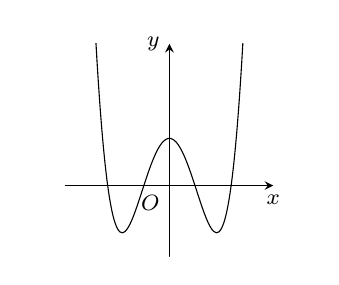
\begin{tikzpicture}[scale=0.6, font=\footnotesize, line join=round, line cap=round, >=stealth]
			\def\a{2} % Hệ số a phải khác 0
			\def\b{-4}
			\def\c{1}
			\draw[->] (-2.2,0) -- (2.2,0) node[below]{$x$};
			\draw[->] (0,-1.5) -- (0,3) node[left]{$y$};
			\draw (0,0)node[below left]{$O$};
			\clip (-3,-1.5)rectangle(3,3);
			\draw[samples=150,smooth,domain=-4:4] plot(\x,{\a*(\x)^4+(\b)*(\x)^2+(\c)});
		\end{tikzpicture}
	}
	\loigiai{
		Đồ thị hàm số có 3 cực trị. Do đó ta loại các hàm số bậc $3$.\\
		Ta có $a>0$ vì nhánh ngoài cùng bên phải đi lên.\\
		Do đó ta chọn hàm số $y=2x^4-4x^2+1$.
	}
\end{ex}
%%==========Câu 32
\begin{ex}%[2H3Y1-1]
	Trong không gian $Oxyz$, cho hai điểm $A(-1;2;1),B(1;1;3)$. Tọa độ của véc tơ $\overrightarrow{AB}$ là
	\choice
	{$(-2;1;-2)$}
	{\True $(2;-1;2)$}
	{ $(0;3;4)$}
	{ $(0;-1;2)$}
	\loigiai{
		Ta có $\overrightarrow{AB}=(2;-1;2)$.}
\end{ex}
%%==========Câu 33
\begin{ex}%[2D2B5-3]
	Khi đặt $t=\log x$ thì phương trình ${{\log }^2}{x^3}-3\log x-1=0$ trở thành phương trình nào sau đây?
	\choice[0.4em]
	{ $t^2-3t-1=0$}
	{ $6t^2-3t-1=0$}
	{ $3t^2-3t-1=0$}
	{\True $9t^2-3t-1=0$}
	\loigiai{
		Ta có\\
		${{\log }^2}{x^3}-3\log x-1=0\Leftrightarrow {{\left( 3\log x \right)}^2}-3\log x-1=0\Leftrightarrow 9{{\log }^2}x-3\log x-1=0$.\\
		Đặt $t=\log x$ thì phương trình trở thành $9t^2-3t-1=0$.}
\end{ex}
%%==========Câu 34
\begin{ex}%[2H2Y2-1]
	Thể tích khối cầu bán kính $R=3a$ là
	\choice[0.4em]
	{\True $V=36\pi {a^3}$}
	{ $V=18\pi {a^3}$}
	{ $V=12\pi {a^3}$}
	{ $V=12\pi {a^2}$}
	\loigiai{
		Ta có\\
		Thể tích khối cầu bán kính $R=3a$ là $V=\dfrac{4}{3}\pi {R^3}=\dfrac{4}{3}\pi {{\left( 3a \right)}^3}=36\pi {a^3}$.}
\end{ex}
%%==========Câu 35
\begin{ex}%[2H3Y3-1]
	Trong không gian $Oxyz,$ cho đường thẳng $\Delta :\left\{ \begin{aligned}
		& x=1-2t \\
		& y=2+t \\
		& z=3 \\
	\end{aligned} \right..$ Một vectơ chỉ phương của đường thẳng $\Delta $ là
	\choice[0.4em]
	{ $\overrightarrow{u_3}=\left( 1;2;3 \right)$}
	{\True $\overrightarrow{u_4}=\left( -2;1;0 \right)$}
	{ $\overrightarrow{u_4}=\left( -2;1;3 \right)$}
	{ $\overrightarrow{u_4}=\left( 2;1;0 \right)$}
	\loigiai{Ta có $\overrightarrow{u_4}=\left( -2;1;0 \right)$ là một véc-tơ chỉ phương của $\Delta$.}
\end{ex}
%%==========Câu 36
\begin{ex}%[2H3B2-3]
	Trong mặt phẳng $Oxyz$ viết phương trình mặt phẳng đi qua $A(1;-1;2)$ và có vec tơ pháp tuyến $\overrightarrow{n}=(2;2;1)$.
	\choice[0.4em]
	{\True $2x+2y+z-2=0$}
	{ $2x+2y+2z+2=0$}
	{ $x-y+2z-2=0$}
	{ $x-y+2z=0$}
	\loigiai{
		Phương trình mặt phẳng đi qua $A(1;-1;2)$và một vectơ pháp tuyến $\overrightarrow{n}=(2;2;1)$ là
		$$2(x-1)+2(y+1)+(z-2)=0\Leftrightarrow 2x+2y+z-2=0.$$
	}
\end{ex}
%%==========Câu 37
\begin{ex}%[Dự án 16 - TT-LuongTai-BacNinh-L12-NH21-22]%[2D4Y1-1]
	Phần ảo của số phức $z = -3 + 4i$ là
	\choice
	{ $3$}
	{ $-3$}
	{\True $4$}
	{ $-4$}
	\loigiai{
		Phần ảo của số phức $z=-3+4i$ là $4$.}
\end{ex}

%%==========Câu 38
\begin{ex}%[Dự án 16 - TT-LuongTai-BacNinh-L12-NH21-22]%[2D3B1-1]
	Tìm hàm số $y = f(x)$ biết rằng $f'(x) = \sin x + 2$ và $f(0) = 1$.
	\choice
	{ $\cos x + 2x + 1$}
	{\True $-\cos x + 2x + 2$}
	{ $-\cos x + 2x + 1$}
	{ $-\cos x + 2x$}
	\loigiai{
		Ta có $f(x) = \displaystyle\int f'(x) \mathrm{\,d}x = \displaystyle\int (\sin x + 2) \mathrm{\,d}x = -\cos x + 2x + C$.\\
		Do $f(0) = 1 \Leftrightarrow 1 = -\cos 0 + 2 \cdot 0 + C \Leftrightarrow C = 2$.\\
		Do đó $f(x) = -\cos x + 2x + 2$.}	
\end{ex}

%%==========Câu 39
\begin{ex}%[Dự án 16 - TT-LuongTai-BacNinh-L12-NH21-22]%[2D2K6-1]
	Tập nghiệm của bất phương trình $\left(4^x - 65 \cdot 2^x + 64 \right)\left[2 - \log_3 \left(x + 3 \right) \right] \ge 0$ có tất cả bao nhiêu số nguyên?
	\choice
	{$2$}
	{$3$}
	{\True $4$}
	{Vô số}
	\loigiai{
		Ta có
		\allowdisplaybreaks
		$\begin{aligned}[t]
			\left(4^x - 65 \cdot 2^x + 64 \right)\left[2 - \log_3 \left(x + 3 \right) \right] \ge 0&\Leftrightarrow \hoac{&\heva{&4^x - 65 \cdot 2^x + 64 \leq 0\\&2 - \log_3 \left(x + 3 \right) \leq 0}\\&\heva{&4^x - 65 \cdot 2^x + 64 \geq 0\\&2 - \log_3 \left(x + 3 \right) \geq 0}} \Leftrightarrow \hoac{&\heva{&1 \leq 2^x \leq 64\\&x \geq 6}\\&\heva{&\hoac{&2^x \geq 64\\&2^x \leq 1}\\&-3 < x \leq 6}}\\
			&\Leftrightarrow \hoac{&\heva{&0 \leq x \leq 6\\&x \geq 6}\\&\heva{&\hoac{&x \geq 6\\&x \leq 0}\\&-3 < x \leq 6}} \Leftrightarrow \hoac{&x = 6\\&-3 < x \leq 0.}
		\end{aligned}$\\
		Vậy tập nghiệm của bất phương trình có $4$ giá trị nguyên.
	}
\end{ex}

%%==========Câu 40
\begin{ex}%[Dự án 16 - TT-LuongTai-BacNinh-L12-NH21-22]%[2D3K2-1]
	Cho hàm số $ f(x)= \heva{& 2x + a &\text{khi}\;\; x \ge  1 \\& 3x^2 + b &\text{khi}\;\; x < 1}$ thỏa mãn $\displaystyle\int\limits_0^2 f(x) \mathrm{\,d}x = 13$. Tính $T = a + b - ab$?
	\choice
	{\True $T=-11$}
	{ $T=-5$}
	{ $T=1$}
	{ $T=-1$}
	\loigiai{
		Để tồn tại $\displaystyle\int\limits_0^2 f(x) \mathrm{\,d}x  \Leftrightarrow f(x)$ liên tục trên đoạn $[0;2]$ $\Leftrightarrow f(x)$ liên tục tại $x = 1$ (vì $f(x)$ liên tục trên các khoảng $(0;1)$ và $(1;2)$) $\Leftrightarrow \lim\limits_{x \to 1^+} f(x) = \lim\limits_{x \to 1^-} f(x) = f(1) \Leftrightarrow a + 2 = b + 3 \Leftrightarrow a = b + 1 \;\;( 1 )$.\\
		Ta có
		\allowdisplaybreaks
		$\begin{aligned}[t]
			\displaystyle\int\limits_0^2 f(x) \mathrm{\,d}x&=\displaystyle\int\limits_0^1 f(x) \mathrm{\,d}x + \displaystyle\int\limits_1^2 f(x) \mathrm{\,d}x = \displaystyle\int\limits_0^1 (3x^2 + b) \mathrm{\,d}x + \displaystyle\int\limits_1^2 (2x + a) \mathrm{\,d}x\\
			&= (x^3 + bx) \Big|_0^1 + (x^2 + ax) \Big|_1^2 = a + b + 4.
		\end{aligned}$\\
		Mà $\displaystyle\int\limits_0^2 f(x) \mathrm{\,d}x = 13 \Rightarrow a + b = 9$ (2).\\\\
		Từ (1) và (2) suy ra $ a = 5$; $b = 4 \Rightarrow T = a + b - ab = -11$.
	}
\end{ex}

%%==========Câu 41
\begin{ex}%[Dự án 16 - TT-LuongTai-BacNinh-L12-NH21-22]%[2D3K3-1]
	\immini{Cho hàm số $ y=f(x)$ liên tục trên $\mathbb{R}$ có đồ thị như hình vẽ. Giả sử diện tích phần kẻ dọc trên hình vẽ có diện tích bằng $a$. Tính theo $a$ giá trị của tích phân $I = \displaystyle\int\limits_{-3}^2 (2x + 1 )f'(x)\mathrm{\,d}x$?
		\choice
		{\True $I = 50 - 2a$}
		{$I = 50 - a$}
		{$I = -30 - 2a$}
		{$I = -30 + 2a$}
	}{\begin{tikzpicture}[>=stealth,line join=round,line cap=round,font=\footnotesize,scale=.8]
			\draw[->] (-2,0)--(.15,0)node[below left]{$O$} --(3.5,0)node[below]{$x$};
			\draw[->] (0,-2) -- (0,5) node[right]{$y$};
			\draw[smooth] plot[domain=-1.45:2.19] (\x,{25/18*(\x)^5-85/36*(\x)^4-26/9*(\x)^3+139/36*(\x)^2+1});   
			\draw[dashed] (-1,0)|-(0,4) (1,0) |- (0,1);
			\fill[pattern=north east lines] (-1,0) -- plot[domain=-1:1] (\x,{25/18*(\x)^5-85/36*(\x)^4-26/9*(\x)^3+139/36*(\x)^2+1}) -- (1,0)--cycle;
			\path 
			(-1,0) node[below] {$-3$}
			(1,0) node[below] {$2$}
			(2,0) node[below right] {$4$}
			(0,1) node[below left] {$2$}
			(0,4) node[right] {$8$};
		\end{tikzpicture}
	}
	\loigiai{
		Từ đồ thị suy ra $S = \displaystyle\int\limits_{-3}^2 f(x)\mathrm{\,d}x = a$ và $ f(-3) = 8$; $f(2) = 2$.\\
		Ta có
		\allowdisplaybreaks
		$\begin{aligned}[t]
			I &= \displaystyle\int\limits_{-3}^2 (2x + 1) f'(x)\mathrm{\,d}x = \displaystyle\int\limits_{-3}^2 (2x + 1)\mathrm{\,d}(f(x)) = (2x + 1)f(x)\Big|_{-3}^2 - 2\displaystyle\int\limits_{-3}^2 f(x)\mathrm{\,d}x\\
			&= 5f(2) + 5f(-3) - 2S = 5 \cdot 2 + 5 \cdot 8 - 2a = 50 - 2a.
		\end{aligned}$\\
		Vậy $I = 50 - 2a$.
	}
\end{ex}

%%==========Câu 42
\begin{ex}%[Dự án 16 - TT-LuongTai-BacNinh-L12-NH21-22]%[2D1K3-1]
	\immini{Cho hàm số $ y = f(x)$ liên tục trên $\mathbb{R}$ và có đồ thị của hàm số $f'(x)$ như hình vẽ bên. Tìm giá trị nhỏ nhất của hàm số $ y = f(x)$ trên đoạn $[-1; 2]$?
		\choice
		{$f(2)$}
		{$1$}
		{$f(-1)$}
		{\True $f(1)$}
	}{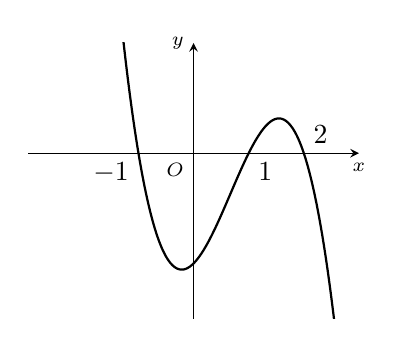
\begin{tikzpicture}[>=stealth,x=1cm,y=1cm,scale=0.7]
			\def\a{-1} % Hệ số a phải khác 0
			\def\b{2}
			\def\c{1}
			\def\d{-2}
			%\draw[color=gray,dash pattern=on 1pt off 1pt,xstep=1.0cm,ystep=1.0cm] (-5.2,-5.2) grid (5.2,5.2);
			\draw[->] (-3,0) -- (3,0)node[below]{\scriptsize $x$};
			\draw[->] (0,-3) -- (0,2) node[left] {\scriptsize $y$};
			\draw (0,0)node[below left]{\scriptsize $O$};
			\clip (-3,-3)rectangle(3,2);
			\draw[thick,samples=150,smooth,domain=-3:3] plot(\x,{\a*(\x)^3+(\b)*(\x)^2+(\c)*\x+(\d)});
			\draw (-1,0) node[below left]{$-1$};
			\draw (1,0) node[below right]{$1$};
			\draw (2,0) node[above right]{$2$};
		\end{tikzpicture}
	}
	\loigiai{
		Từ đồ thị hàm số $ f'(x) \Rightarrow f'(x) = 0 \Leftrightarrow \hoac{&x = -1\\&x = 1\\&x = 2.}$\\
		Bảng biến thiên
		\begin{center}
			
\begin{tikzpicture}
				\tkzTabInit[nocadre=true,lgt=1.2,espcl=3]
				{$x$/1.2,$f’(x)$/1.2,$f(x)$/2.5}
				{$-\infty$,$-1$,$1$,$2$,$+\infty$}
				\tkzTabLine{ ,+,z,-,z,+,z,-, }
				\tkzTabVar{-/$-\infty$,+/$f(-1)$,-/$f(1)$,+/$f(2)$,-/$-\infty$}
			\end{tikzpicture}
		\end{center}
		Từ bảng biến thiên suy ra giá trị nhỏ nhất của hàm số $y = f(x)$ trên đoạn $[-1;2]$ là $f(1)$.
	}	
\end{ex}

%%==========Câu 43
\begin{ex}%[Dự án 16 - TT-LuongTai-BacNinh-L12-NH21-22]%[1H3B3-3]
	Cho hình chóp $S.ABC$ có đáy $ABC$ là tam giác đều cạnh bằng $2a$. Tam giác $SAB$ là tam giác vuông cân tại $S$ và nằm trong mặt phẳng vuông góc với đáy. Tính góc giữa đường thẳng $SC$ và mặt phẳng $ABC$?
	\choice
	{$60^\circ$}
	{\True $30^\circ$}
	{$45^\circ$}
	{$90^\circ$}
	\loigiai{
		\immini{Gọi $H$ là trung điểm của $AB$.\\
			Do $\triangle SAB$ là tam giác vuông cân tại $S$ và nằm trong mặt phẳng vuông góc với đáy nên ta có: $SH = \dfrac{AB}{2} = a$ và $S H\perp (ABC)$.\\
			Suy ra $(\widehat{SC,(ABC)}) = \widehat{SCH}$.\\
			$\triangle ABC$ là tam giác đều cạnh bằng $2a$ nên $CH = a\sqrt{3}$.\\
			Xét $\triangle SCH$ vuông tại $H$ có $\tan \widehat{SCH} = \dfrac{SH}{CH} = \dfrac{1}{\sqrt{3}}$.\\
			Suy ra $(\widehat{SC,(ABC)}) = 30^\circ$.
		}{\begin{tikzpicture}[line join=round,line cap=round,line width=.6pt,font=\footnotesize,scale=1.0]
				\coordinate[label=left:$A$] (A) at (0,0);
				\coordinate[label=below left:$B$] (B) at (2.5,-1);
				\coordinate[label=right:$C$] (C) at (4,0);
				\coordinate[label=below left:$H$] (H) at ($(A)!.5!(B)$); % Thay đổi số 1/2 để đổi vị trí điểm H
				\coordinate[label=above left:$S$] (S) at ($(H)+(90:4)$);
				\draw (A)--(B)--(C)--(S)--cycle (H)--(S)--(B);
				\draw[dashed] (A)--(C)--(H);	
				\fill (C)circle(1.5pt) (B)circle(1.5pt) (A)circle(1.5pt) (S)circle(1.5pt) (H)circle(1.5pt);
			\end{tikzpicture}
		}
	}
\end{ex}
%%==========Câu 44
\begin{ex}%[Dự án 16 - TT-LuongTai-BacNinh-L12-NH21-22]%[1H3K5-3]
	\immini{Cho lăng trụ tam giác đều $ABC.A'B'C'$ có cạnh đáy bằng $4a$. Góc giữa hai mặt phẳng $(A'BC)$ và $(ABC)$ bằng $30^\circ$. Gọi $M$ là trung điểm của cạnh $AB$. Tính khoảng cách từ điểm $M$ đến mặt phẳng $(A'BC)$?\\
		\choice
		{\True $\dfrac{a\sqrt{3}}{2}$}
		{ $3a$}
		{ $a\sqrt{3}$}
		{ $\dfrac{3a}{2}$}
	}{\begin{tikzpicture}[line join=round,line cap=round,line width=.6pt,font=\footnotesize,scale=0.7]
			\coordinate[label=left:$A$] (A) at (0,0);
			\coordinate[label=below left:$B$] (B) at (2,-1);
			\coordinate[label=right:$C$] (C) at (5,0);
			\coordinate[label=left:$A'$] (A1) at ($(A)+(90:4)$);
			\coordinate[label=above:$B'$] (B1) at ($(B)-(A)+(A1)$);
			\coordinate[label=right:$C'$] (C1) at ($(C)-(A)+(A1)$);
			\coordinate[label=below left:$M$] (M) at ($(A)!0.5!(B)$);
			\draw (A1)--(A)--(B)--(C)--(C1)--(A1)--(B1)--(C1) (B)--(B1);
			\draw[dashed] (A)--(C) (A1)--(B) (A1)--(C);
			\fill (A)circle(1.5pt) (B)circle(1.5pt) (C)circle(1.5pt) (A1)circle(1.5pt) (B1)circle(1.5pt) (C1)circle(1.5pt) (M)circle(1.5pt);
	\end{tikzpicture}}
	\loigiai{
		\immini{Gọi $N$ là trung điểm của $BC$.\\
			Do $ABC.A'B'C'$ là lăng trụ tam giác đều nên \\ $\heva{&BC \perp AN\\&BC \perp AA'} \Rightarrow BC \perp (A'AN)$ và $AN = 2a\sqrt{3}$. \\Từ đó ta có: $\widehat{\left(A'BC \right),\left(ABC \right)} = \widehat{A'NA} = 30^\circ$.\\
			Gọi $H$ là hình chiếu của $A$ trên $A'N$, do $BC \perp \left( A'AN \right)$ nên $$\heva{&AH \perp AN\\&AH \perp BC} \Rightarrow AH \perp \left( A'BC \right) \Rightarrow \mathrm{\,d}\left( A,\left( A'BC \right) \right) = AH.$$
		}{\begin{tikzpicture}[line join=round,line cap=round,line width=.6pt,font=\footnotesize,scale=0.8]
				\coordinate[label=left:$A$] (A) at (0,0);
				\coordinate[label=below left:$B$] (B) at (2,-1);
				\coordinate[label=right:$C$] (C) at (5,0);
				\coordinate[label=left:$A'$] (A1) at ($(A)+(90:4)$);
				\coordinate[label=above:$B'$] (B1) at ($(B)-(A)+(A1)$);
				\coordinate[label=right:$C'$] (C1) at ($(C)-(A)+(A1)$);
				\coordinate[label=below left:$M$] (M) at ($(A)!0.5!(B)$);
				\coordinate[label=below right:$N$] (N) at ($(C)!0.5!(B)$);
				\coordinate[label=above:$H$] (H) at ($(A1)!0.5!(N)$);
				\foreach \x/\dinh/\y in {A/N/B,A/H/N} \draw[fill = gray!50] ($(\dinh)!5pt!(\x)$)--($(\dinh)!5pt!(\x)+(\dinh)!5pt!(\y)-(\dinh)$)--($(\dinh)!5pt!(\y)$)--(\dinh)--cycle; 
				\draw (A1)--(A)--(B)--(C)--(C1)--(A1)--(B1)--(C1) (B)--(B1) (A1)--(B);
				\draw[dashed] (A)--(C) (A1)--(C) (A)--(N) (A)--(H) (A1)--(N);
				\fill (A)circle(1.5pt) (B)circle(1.5pt) (C)circle(1.5pt) (A1)circle(1.5pt) (B1)circle(1.5pt) (C1)circle(1.5pt) (M)circle(1.5pt) (N)circle(1.5pt) (H)circle(1.5pt);
		\end{tikzpicture}}
		\noindent Xét $\triangle AHN$ vuông tại $H$ có: $AH = AN \cdot \sin \widehat{ANA'} = a\sqrt{3}$.\\
		Suy ra $\mathrm{\,d}\left( A,\left(A'BC\right) \right) = a\sqrt{3}$.\\
		Mặt khác, $M$ là trung điểm của cạnh $AB$ nên
		$\mathrm{\,d}\left( M,\left(A'BC \right) \right) = \dfrac{1}{2}d\left( A,\left( A'BC \right) \right) = \dfrac{a\sqrt{3}}{2}.$
	}
\end{ex}
%%==========Câu 45
\begin{ex}%[2H1K3-2]
	Cho lăng trụ $ABC.A'B'C'$, gọi $M$, $N$ lần lượt là trung điểm của cạnh $AA'$ và $BC$. Biết khối tứ diện $A.MNB$ có thể tích là $3a^3$. Tính thể tích lăng trụ $ABC.A'B'C'$
	\choice
	{ $9a^3$}
	{ $12a^3$}
	{\True $36a^3$}
	{ $18a^3$}
	\loigiai{
		\immini{Gọi $V$ là thể tích lăng trụ $ABC.A'B'C'$.\\
			Ta có $V_{M.ABN}=\dfrac{1}{2}V_{M.ABC}=\dfrac{1}{2}\cdot \dfrac{1}{2}V_{A'. ABC}=\dfrac{1}{4}\cdot \dfrac{1}{3}V=\dfrac{1}{12}V$.\\
			Suy ra $V=12V_{A.MNB}=36a^3$.}{
	\begin{tikzpicture}[scale=.7, font=\footnotesize, line join=round, line cap=round, >=stealth]
		\def\ac{4} % cạnh AC
		\def\ab{2} % cạnh AB
		\def\ben{4} % cạnh bên
		\def\gocnghieng{75} % góc nghiêng cạnh bên
		\def\gocA{50} % góc A của đáy
		\coordinate[label=left:$A$] (A) at (0,0);
		\coordinate[label=right:$C$] (C) at (\ac,0);
		\coordinate[label=below left:$B$] (B) at (-\gocA:\ab);
		\coordinate[label=left:$A'$] (A') at ($(A)+(\gocnghieng:\ben)$);
		\coordinate[label=below left:$B'$] (B') at ($(B)-(A)+(A')$);
		\coordinate[label=right:$C'$] (C') at ($(C)-(A)+(A')$);
		\coordinate[label=left:$M$] (M) at ($(A)!.5!(A')$);
		\coordinate[label=below right:$N$] (N) at ($(C)!.5!(B)$);
		\draw (A')--(A)--(B)--(C)--(C')--(A')--(B')--(C') (M)--(B)--(B');
		\draw[dashed] (A)--(C) (A)--(N)--(M)--(C);
		\foreach \diem in {A,B,C,N,A',B',C',M} \fill (\diem)circle(1.5pt);
	\end{tikzpicture}
		
	}}
\end{ex}
%%==========Câu 46
\begin{ex}%[2D1G5-3]
	\immini[thm]{Cho hàm số $ y=f(x)$ là hàm số bậc ba có đồ thị như hình vẽ. Tìm tất cả các giá trị của tham số $ m$ sao cho phương trình $ f(\sin x)=f(m+1)$ có nghiệm?
	\choice
	{ $-1\le m\le3$}
	{ $-2\le m\le0$}
	{\True $-3\le m\le1$}
	{ $-2\le m\le2$}}
{
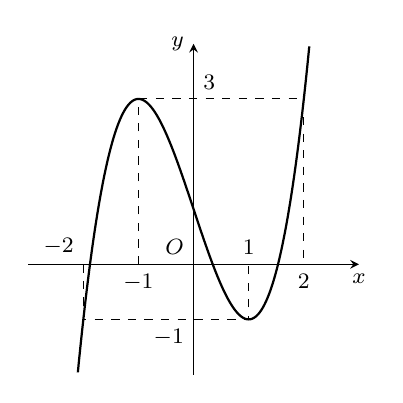
\begin{tikzpicture}[>=stealth,x=1cm,y=1cm,scale=0.7, font=\footnotesize]
	\def\a{1} % Hệ số a phải khác 0
	\def\b{0}
	\def\c{-3}
	\def\d{1}
	\draw[->] (-3,0) -- (3,0)node[below]{$x$};
	\draw[->] (0,-2) -- (0,4) node[left] {$y$};
	\draw (0,0)node[above left]{$O$};
	\draw (1,0)node[above]{$1$} (-2,0)node[above left]{$-2$} (-1,0)node[below]{$-1$} (2,0)node[below]{$2$} (0,3)node[above right]{$3$} (0,-1)node[below left]{$-1$};
	\draw[thick,samples=150,smooth,domain=-2.1:2.1] plot(\x,{\a*(\x)^3+(\b)*(\x)^2+(\c)*\x+(\d)});
	\draw[dashed] (-2,0)--(-2,-1)--(1,-1)--(1,0) (-1,0)--(-1,3)--(2,3)--(2,0);
\end{tikzpicture}
}
	\loigiai{
	Ta có $\sin x\in [-1;1]$ nên $ f(\sin x)\in [-1;3]$.\\
		Do đó $ f(m+1)\in [-1;3]$ nên $-2\le m+1\le2\Leftrightarrow -3\le m\le1$.}
\end{ex}
%%==========Câu 47
\begin{ex}%[2D2G5-5]
	Có tất cả bao nhiêu số nguyên dương $ y$ sao cho tồn tại số thực $ x\in (1;8)$ thỏa mãn phương trình $(x-1)(2\mathrm{e}^x-y^2)=y(\mathrm{e}^x-x^2)$?
	\choice
	{ $11$}
	{ $14$}
	{ $12$}
	{\True $13$}
	\loigiai{
		Xét $ f(x)=(x-1)(2\mathrm{e}^x-y^2)-y(\mathrm{e}^x-x^2)$ trên $(1;8)$ với $ y$ là tham số.\\
		Ta có $f'(x)=2x\mathrm{e}^x-y\mathrm{e}^x-y^2+2yx=(\mathrm{e}^x+y)(2x-y)\Rightarrow f'(x)=0\Leftrightarrow x=\dfrac{y}{2}$.\\
		Nhận thấy $ f(1)=-y(e-1)<0$ (vì $ y$ nguyên dương).\\
		Và $ f(8)=7(2\mathrm{e}^8-y^2)-y(\mathrm{e}^8-64)=-7y^2-(\mathrm{e}^8-64)y+14\mathrm{e}^8$.\\
		\textbf{Trường hợp 1:} $\dfrac{y}{2}\le1\Leftrightarrow y\le2\Rightarrow f'(x)>0$. \\
		Bảng biến thiên
		\begin{center}
			
\begin{tikzpicture}[>=stealth]
				\tkzTabInit[nocadre=true,lgt=1.5,espcl=7,deltacl=0.5]{$x$/.7 ,$y'$/.7,$y$/2}
				{$1$ , $8$}
				\tkzTabLine{ , + , }
				\tkzTabVar{-/$-\infty$ , +/$+\infty$}
			\end{tikzpicture}
		\end{center}
		Suy ra $ f(8)>0\Leftrightarrow -7y^2-(\mathrm{e}^8-64)y+14\mathrm{e}^8>0\Rightarrow 0<y<13\cdot 85$.\\
		Do vậy $0<y\le2\Rightarrow y\in \{1;2\}$.\\
		\textbf{Trường hợp 2:} $\dfrac{y}{2}\ge8\Leftrightarrow y\ge16\Rightarrow f'(x)<0\Rightarrow f(8)<f(1)<0$.\\
		Khi đó phương trình vô nghiệm trên $(1;8)$.\\
		\textbf{Trường hợp 3:} $1<\dfrac{y}{2}<8\Leftrightarrow 2<y<16\Rightarrow x_{\text{CT}}=\dfrac{y}{2}$. \\
		Bảng biến thiên
		\begin{center}
			
\begin{tikzpicture}[>=stealth]
				\tkzTabInit[nocadre=true,lgt=1,espcl=4,deltacl=0.75]{$x$/1 ,$y'$/1,$y$/2.5}
				{$1$ , $\dfrac{y}{2}$ , $8$}
				\tkzTabLine{ , - , $0$ , + , }
				\tkzTabVar{+/$f(1)$ , -/$f\left( \dfrac{y}{2}\right) $ , +/$f(8)$}
			\end{tikzpicture}
		\end{center}
		Suy ra $ f(8)>0\Leftrightarrow -7y^2-(\mathrm{e}^8-64)y+14\mathrm{e}^8>0\Rightarrow 0<y<13\cdot 85$.\\
		Do vậy $2<y<13{,}85\Rightarrow y\in \{3;4;\ldots ;13\}$.\\
		Vậy có $13$ giá trị nguyên dương $ y$ thỏa mãn.}
\end{ex}
%%==========Câu 48
\begin{ex}%[2D3G3-1]
	Cho hàm số $ f(x)=x^3+bx^2+cx+d$ với $ b$, $ c$, $ d$ là các số thực. Biết hàm số $ g(x)=f(x)+2f'(x)+3f''(x)$ có hai giá trị cực trị là $-6$ và $42$. Tính diện tích hình phẳng giới hạn bởi các đường $ y=\dfrac{f(x)+f'(x)+f''(x)}{g(x)+18}$ và $ y=1$
	\choice
	{\True $\ln5$}
	{ $\ln7$}
	{ $2\ln6$}
	{ $2\ln5$}
	\loigiai{
		Hàm số $ f(x)$ là hàm số bậc $3$ nên $ g(x)$ là hàm số bậc $3$ suy ra $g'(x)$ là hàm số bậc hai.\\
		Ta có $3f^{(3)}(x)=3\cdot 3!=18$;\\
		$g'(x)=f'(x)+2f''(x)+18$ có hai nghiệm $x_1$, $x_2$ (giả sử $x_1<x_2$) và $ g(x_1)=42$, $ g(x_2)=-6$.\\
		Xét phương trình tìm cận của tích phân để tính diện tích
\begin{center}
			$\dfrac{f(x)+f'(x)+f''(x)}{g(x)+18}=1\Leftrightarrow \dfrac{f'(x)+2f''(x)+18}{g(x)+18}=0$.
\end{center}
		Suy ra $f'(x)+2f''(x)+18=0\Leftrightarrow g'(x)=0\Leftrightarrow \hoac{ &x=x_1\\ &x=x_2.} $\\
		Diện tích hình phẳng \begin{center}
			$S=\displaystyle\int\limits_{x_1}^{x_2}{\left|\dfrac{f(x)+f'(x)+f''(x)}{g(x)+18}-1\right|\mathrm{\,d}x}=\displaystyle\int\limits_{x_1}^{x_2}{\left|\dfrac{{g}'(x)}{g(x)+18}\right|\mathrm{\,d}x}=\left|\displaystyle\int\limits_{x_1}^{x_2}{\dfrac{{g}'(x)}{g(x)+18}\mathrm{\,d}x}\right|$.
		\end{center}
		Đặt $ t=g(x)+18\Rightarrow \mathrm{\,d}t=g'(x)\mathrm{\,d}x$. Đổi cận $\heva{ &x=x_1\Rightarrow {t_1}=g(x_1)+18\\ &x=x_2\Rightarrow {t_2}=g(x_2)+18.} $\\
		Do đó $S=\left|\displaystyle\int\limits_{60}^{12}\dfrac{\mathrm{\,d}t}{t}\right|=\left|\ln t\biggl|_{60}^{12}\right|=\left|\ln12-\ln60\right|=\left|\ln\dfrac{12}{60}\right|=|-\ln5|=\ln5$.}
\end{ex}
%%==========Câu 49
\begin{ex}%[2H3G3-7]
	Trong không gian $Oxyz$, cho điểm $A(2;4;-2)$ và mặt phẳng $(P)\colon (m^2+1)x+(m^2-1)y+2mz+4=0$. Biết rằng, khi tham số thay đổi thì mặt phẳng $(P)$ luôn tiếp xúc với hai mặt cầu cố định cùng đi qua $A$ là $(S_1)$, $(S_2)$. Gọi $M$ và $N$ lần lượt là hai điểm nằm trên $(S_1)$ và $(S_2)$. Tìm giá trị lớn nhất của $MN$.
	\choice
	{ $16\sqrt{2}$}
	{\True $8+8\sqrt{2}$}
	{ $8\sqrt{2}$}
	{ $8+6\sqrt{2}$}
	\loigiai{
		Đặt $ m=\tan t$. Khi đó 
		\allowdisplaybreaks
		\begin{eqnarray*}
			&& (P)\colon (\tan^2t+1)\cdot x+(\tan ^2t-1)\cdot y+2\tan t\cdot z+4=0\\
			&\Leftrightarrow& (P)\colon x-\cos 2ty+\sin 2tz+2\cos 2t+2=0.
		\end{eqnarray*}
		Gọi $I(a;b;c)$ và $R$ lần lượt là tâm và bán kính mặt cầu tiếp xúc với $(P)$ với $R$ không đổi.\\
		Khi đó
\begin{center}
			$R=\mathrm{d}\left(I,\left(P\right)\right)=\dfrac{\left|a-\cos 2tb+\sin 2tc+2\cos 2t+2\right|}{\sqrt{2}}=\dfrac{|a+(2-b)\cos 2t+\sin 2tc+2|}{\sqrt{2}}$.
\end{center}
		Để $R$ không đổi khi $ t$ thay đổi $\Leftrightarrow \heva{ &b=2\\ &c=0} \Rightarrow I(a;2;0)$.\\
		Khi đó $ \mathrm{d}\left(I,\left(P\right)\right)=\dfrac{\left|a+2\right|}{\sqrt{2}}=R$ và mặt cầu qua $A(2;4;-2)$.\\
		Nên $I{{A}^2}={R^2}\Leftrightarrow \left(\dfrac{a+2}{\sqrt{2}}\right)^2=\left(a-2\right)^2+8\Leftrightarrow \hoac{ &a=2,R_1=2\sqrt{2}\\ &a=10,R_2=6\sqrt{2}.} $\\
		Khi đó $MN_{\max}=I_1I_2+R_1+R_2=8+8\sqrt{2}$.}
\end{ex}
%%==========Câu 50
\begin{ex}%[2D1G2-6]
	Cho hàm số $ f(x)=2x^3+bx^2+cx+d$ thỏa mãn $4b+2c+d+16<0$ và $9b-3c+d>54$. Hàm số $ y=|f(x)|$ có tất cả bao nhiêu điểm cực trị?
	\choice
	{ $2$}
	{ $3$}
	{\True $5$}
	{ $4$}
	\loigiai{
		Ta có $ f(x)=2x^3+bx^2+cx+d\Rightarrow f(x)$ liên tục trên $\mathbb R$.\\
		Ta có $\heva{ &\lim\limits_{x\to-\infty}f(x)=\lim\limits_{x\to-\infty}(2x^3+bx^2+cx+d)=-\infty\\ &f(-3)=-54+9b-3c+d>0\\ &f(2)=4b+2c+d+16<0\\ &\lim\limits_{x\to+\infty}f(x)=\lim\limits_{x\to+\infty}(2x^3+bx^2+cx+d)=+\infty.} $\\
		Ta có $\lim\limits_{x\to-\infty}f(x)\cdot f(-3)<0$, $ f(-3)\cdot f(2)<0$, $\lim\limits_{x\to+\infty}f(x)\cdot f(2)<0$ nên theo tính chất hàm liên tục thì phương trình $ f(x)=0$ và ít nhất ba nghiệm và $ f(x)$ là hàm bậc ba nên phương trình $ f(x)=0$ sẽ có ba nghiệm. Do đó hàm số $ f(x)$ có hai điểm cực trị.\\
		$\Rightarrow $ Hàm số $|f(x)|$ có $5$ điểm cực trị.
	}
\end{ex}


\Closesolutionfile{ans}